\documentclass[12pt]{article}


% ----------------- PAQUETES -----------------
\usepackage[utf8]{inputenc}
\usepackage[spanish]{babel}
\usepackage[margin = 2.54cm]{geometry}
\usepackage{graphicx}
\usepackage{enumitem}
\usepackage{parskip}
\usepackage{bm}
\usepackage{amsmath}
\usepackage[x11names,table]{xcolor}


% ----------------- CONFIGURACIONES -----------------
% ----------------- UTILIDADES PARA DAR UN MEJOR FORMATO DE DOCUMENTO -----------------  


\definecolor{azul}{rgb}{0.0039, 0.3098, 0.6196}


% Formato para el indice general ...........
\makeatletter
    \renewcommand{\@dotsep}{1.5}
    \renewcommand{\l@section}{\@dottedtocline{1}{1.5em}{2.3em}}
    \renewcommand{\l@subsection}{\@dottedtocline{2}{3.8em}{3.2em}}
    \renewcommand{\l@subsubsection}{\@dottedtocline{3}{7.0em}{4.1em}}
\makeatother

% --------- COMANDOS PERSONALIZADOS PARA LA PORTADA DE LAS TAREAS, TRABAJOS Y PROYECTOS ---------

\newcommand{\rutaLogo}[1]{\newcommand{\RutaLogo}{#1}}
\newcommand{\tema}[1]{\newcommand{\Tema}{#1}}
\newcommand{\etiquetaAutores}[1]{\newcommand{\EtiquetaAutores}{#1}}
\newcommand{\alumno}[1]{\newcommand{\Alumno}{#1}}
\newcommand{\materia}[1]{\newcommand{\Materia}{#1}}
\newcommand{\docente}[1]{\newcommand{\Docente}{#1}}
\newcommand{\ciclo}[1]{\newcommand{\Ciclo}{#1}}
\newcommand{\fecha}[1]{\newcommand{\Fecha}{#1}}
\newcommand{\periodo}[1]{\newcommand{\Periodo}{#1}}

\definecolor{celeste}{HTML}{94E4F1}


% ----------------- PORTADA -----------------
\rutaLogo{../../../docs/img/logo-ista.png}
\tema{\\ \vspace{0.8cm} Guía Practica - Integrales \\ \vspace{1.5cm}}
\etiquetaAutores{Alumno: }
\alumno{Eduardo Mendieta \vspace{0.8cm}}
\materia{Matemática \vspace{0.8cm}}
\docente{Lcda. Vilma Duchi, Mgtr. \vspace{0.8cm}}
\ciclo{Primer ciclo \vspace{0.8cm}}
\fecha{06/09/2024 \vspace{0.8cm}}
\periodo{Abril 2024 - Agosto 2024}


\begin{document}
    \begin{titlepage}

    \centering

    \includegraphics[width=0.11\textwidth]{\RutaLogo} 

    \vspace{0.3cm}
    \textcolor{azul}{\Large \textbf{Instituto Superior Universitario Tecnológico del Azuay \\}}
    \vspace{0.3cm}
    \textcolor{azul}{\Large \textbf{Tecnología Superior en Big Data}}
    
    % 1. ---------------- TEMA -------------------------
    
    {\Large\textbf{\Tema}}
    
    % 2. ---------------- AUTOR(ES) -------------------------
    \textcolor{azul}{\large \textbf{\EtiquetaAutores} \\}
    \vspace{0.3cm}
    {\large \Alumno}

    % 3. ---------------- MATERIA -------------------------
    \textcolor{azul}{\large \textbf{Materia:} \\}
    \vspace{0.3cm}
    {\large \Materia}


    % 3. ---------------- DOCENTE -------------------------
    \textcolor{azul}{\large \textbf{Docente:} \\}
    \vspace{0.3cm}
    {\large \Docente}


    % 3. ---------------- Ciclo -------------------------
    \textcolor{azul}{\large \textbf{Ciclo:} \\}
    \vspace{0.3cm}
    {\large \Ciclo}


    % 3. ---------------- FECHA -------------------------
    \textcolor{azul}{\large \textbf{Fecha:} \\}
    \vspace{0.3cm}
    {\large \Fecha}

    % 3. ---------------- PERIODO -------------------------
    \textcolor{azul}{\large \textbf{Periodo Académico:} \\}
    \vspace{0.3cm}
    {\large \Periodo}
 
\end{titlepage}


    \section*{\centering Guía Practica - Integrales} \vspace{0.5cm}

    \textbf{Resolver las siguientes integrales: } \vspace{0.5cm}

    \begin{itemize}
        \item \textbf{Ejercicio 1: La obra arquitectónica en forma de arco catenario es el Gateway Arch de San Luis(Missouri) diseñada por el arquitecto finlandes Eero Saarinen, este arco tiene como ecuación la siguiente expresión:}
            \[y = 693.85 - 68.76 \cdot \left(\frac{e^{0.0100333x} + e^{-0.0100333x}}{2}\right)\]
        
            \begin{enumerate}
                \item Ingrese dicha ecuación en GeoGebra y obtenga su respectiva gráfica:
                    \begin{figure}[h!]
                        \centering
                        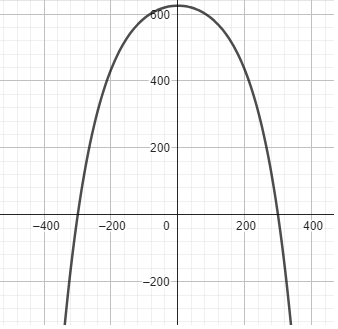
\includegraphics[width=0.4\textwidth]{img/t6-ej1-1.png}
                    \end{figure}
                
                \item Obtén las raíces (puntos de corte con el eje x ) para obtener los extremos del intervalo:
                    \begin{figure}[h!]
                        \centering
                        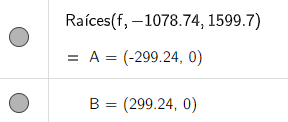
\includegraphics[width=0.4\textwidth]{img/t6-ej1-2.png}
                    \end{figure}

                    \newpage
                    \begin{figure}[h!]
                        \centering
                        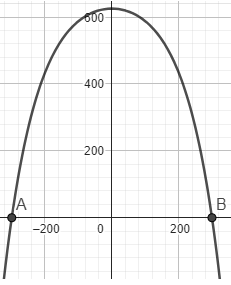
\includegraphics[width=0.3\textwidth]{img/t6-ej1-3.png}
                    \end{figure}
                
                \item ¿Cuál es la anchura de ese intevalo?
                     \[anchura = 299.24 – (- 299.24)= 598.48\]
                
                \item Con el comando \texttt{SumaSuperior} divide a ese intervalo de acuerdo a la siguiente tabla y anota el valor de dicha suma:
                    \begin{table}[h]
                        \centering
                        \begin{tabular}{|l|l|}
                            \hline
                            \textbf{Número de rectángulos} & \textbf{Valor del área} \\
                            \hline
                             4 & 346225.2 \\
                            \hline
                             10 & 310921.52 \\
                            \hline
                             100 & 281319.96 \\
                            \hline
                             1000 & 277993.78 \\
                            \hline
                             10000 & 277657.48 \\
                            \hline
                             100000 & 277657.48 \\
                            \hline
                        \end{tabular}
                    \end{table}

                    \begin{figure}[h!]
                        \centering
                        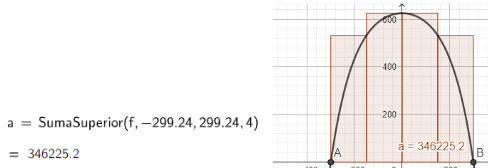
\includegraphics[width=0.7\textwidth]{img/t6-ej1-4.png}
                    \end{figure}

                    \newpage
                    \begin{figure}[h!]
                        \centering
                        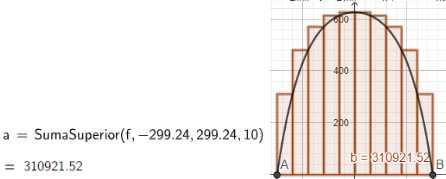
\includegraphics[width=0.7\textwidth]{img/t6-ej1-5.png}
                    \end{figure}
                    \begin{figure}[h!]
                        \centering
                        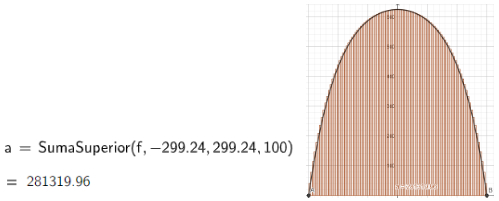
\includegraphics[width=0.7\textwidth]{img/t6-ej1-6.png}
                    \end{figure}
                    \begin{figure}[h!]
                        \centering
                        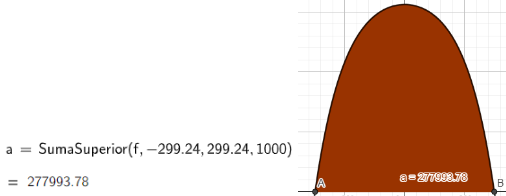
\includegraphics[width=0.7\textwidth]{img/t6-ej1-7.png}
                    \end{figure}
                    \begin{figure}[h!]
                        \centering
                        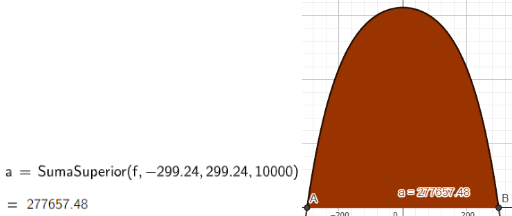
\includegraphics[width=0.7\textwidth]{img/t6-ej1-8.png}
                    \end{figure}
                    \newpage
                    \begin{figure}[h!]
                        \centering
                        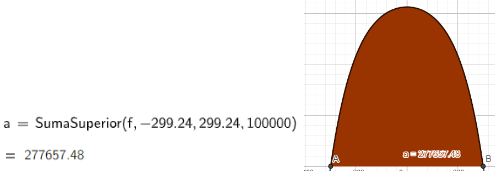
\includegraphics[width=0.7\textwidth]{img/t6-ej1-9.png}
                    \end{figure}
                
                \item ¿Cuál valor de número de rectángulo se aproxima mejor el área bajo esa curva? Para ello utilizar el comando \texttt{Integral:}
                    \begin{table}[h]
                        \centering
                        \begin{tabular}{|l|l|}
                            \hline
                            \textbf{Valor de área con el comando Integral} & 277620.08\\
                            \hline
                            \textbf{Valor de área con el comando SumaSuperior} & 277657.48 - 100000 rectángulos\\
                            \hline                          
                        \end{tabular}
                    \end{table}
                    \begin{figure}[h!]
                        \centering
                        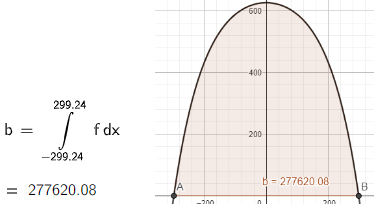
\includegraphics[width=0.7\textwidth]{img/t6-ej1-10.png}
                    \end{figure}
            \end{enumerate}
        

        \newpage
        \item \textbf{Ejercicio 2: Hallar el área de la región limitada por las curvas:}\vspace{0.5cm}
            \begin{enumerate}
                \hrule
                \item \[\bm{y = 2 - x^2, y = x}\]
                    \[\bm{\int_{-2}^{1} 2 - x^2 - x \, dx} = \left[2x - \frac{x^3}{3} - \frac{x^2}{2}\right]_{-2}^{1} = ...\]
                    \[... = 2(1) - \frac{(1)^3}{3} - \frac{(1)^2}{2} - 2(-2) + \frac{(-2)^3}{3} + \frac{(-2)^2}{2} = 2 -\frac{1}{3} - \frac{1}{2} + 4 - \frac{8}{3} + 2 = \bm{\frac{9}{2}u^2}\]
                    \begin{figure}[h!]
                        \centering
                        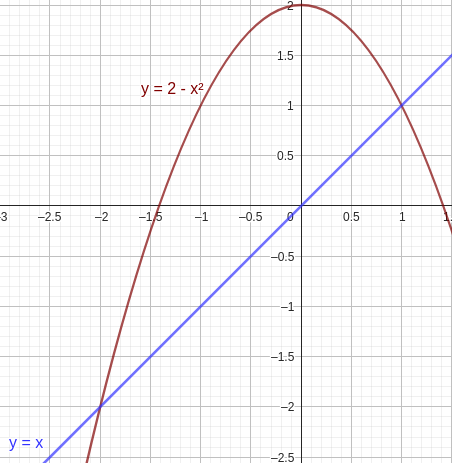
\includegraphics[width=0.4\textwidth]{img/t6-ej2-1.png}
                    \end{figure}
            
                \hrule
                \item \[\bm{y = 4x - x^2, y = 0, x = 1, x = 3}\]
                    \[\bm{\int_{1}^{3} 4x - x^2 \, dx} = \left[2x^2 - \frac{x^3}{3}\right]_{1}^{3} = ...\]
                    \[... = 2(3)^2 - \frac{(3)^3}{3} - 2(1)^2 + \frac{(1)^3}{3} = 18 - 9 - 2 +\frac{1}{3} = \bm{\frac{22}{3}u^2}\]
                    \begin{figure}[h!]
                        \centering
                        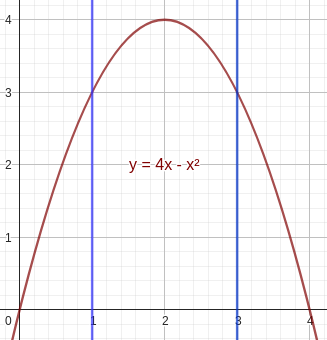
\includegraphics[width=0.3\textwidth]{img/t6-ej2-2.png}
                    \end{figure}


                \newpage\hrule
                \item \[\bm{y = \sqrt{x - 4}, y = 0, x = 8}\]
                    \[\bm{\int_{4}^{8} (x - 4)^{1/2} \, dx} = \int_{4}^{8} (v)^{1/2} \, dv = \left[\frac{2}{3}v^{3/2}\right]_{4}^{8} = ...\]
                    \[... = \left[\frac{2}{3}(x - 4)^{3/2}\right]_{4}^{8} = \frac{2}{3}(4)^{3/2} - \frac{2}{3} = \bm{\frac{14}{3}u^2}\]
                    \begin{figure}[h!]
                        \centering
                        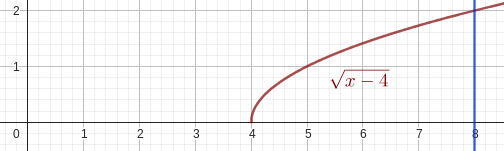
\includegraphics[width=0.6\textwidth]{img/t6-ej2-3.png}
                    \end{figure}

                \hrule
                \item \[\bm{y = x^2 - 4x + 3, x - y - 1 = 0}\]
                    \[\bm{\int_{1}^{4} - x^2 + 5x - 4 \, dx} = \left[- \frac{x^3}{3} + \frac{5x^2}{2} - 4x\right]_{1}^{4} = ...\]
                    \[... = - \frac{(4)^3}{3} + 5\frac{(4)^2}{2} - 4(4) + \frac{1}{3} - \frac{1}{2} + 4 = - \frac{64}{3} + 40 - 16 + \frac{1}{3} - \frac{1}{2} + 4 = \bm{\frac{13}{2}u^2}\]
                    \begin{figure}[h!]
                        \centering
                        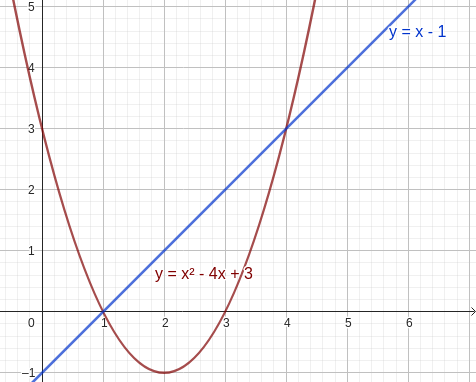
\includegraphics[width=0.5\textwidth]{img/t6-ej2-4.png}
                    \end{figure}
            
                \newpage\hrule
                \item \[\bm{y = \sqrt{2x}, y = 2x - 4, x = 0}\]
                    \[\bm{\int_{}^{}  \, dx} = \left[\right]_{}^{} = ...\]
                    \[... =   = \bm{u^2}\]
                    \begin{figure}[h!]
                        \centering
                        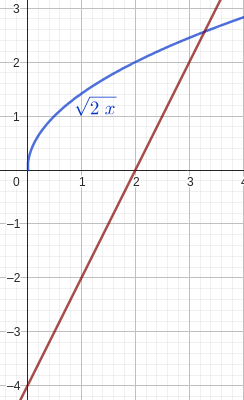
\includegraphics[width=0.4\textwidth]{img/t6-ej2-5.png}
                    \end{figure}

                \hrule
                \item \[\bm{y^2 - 2x = 0, y^2 + 4x - 12 = 0}\]

                \hrule
                \item \[\bm{y^2 = x + 2, y = x - 4}\]

                \hrule
                \item \[\bm{y = x^2, y = - x^2 + 4x}\]

                \hrule
                \item \[\bm{y = x + 6, y = x^3, y = - \frac{2x}{4}}\]
                
                \hrule
                \item \[\bm{y = \left|x - 1\right|, y = x^2 - 3}\]
                
                \hrule
                \item \[\bm{y = x^3 + 3x^2, y = x}\]
                
                \hrule
                \item \[\bm{y = x^3 - 6x^2 + 8x, y = x^2 - 4x}\]

            \end{enumerate}
        
        \item \textbf{Ejercicio 3: Calcular el volúmen del sólido generado por la rotación de la región $\bm{R}$ al rededor del eje indicado; siendo $\bm{R}$ la región limitada por las curvas, cuyas ecuaciones se dan a continuación:} \vspace{0.5cm}
            \begin{enumerate}[label=\alph*.]
                \hrule
                \item \[\bm{y = 2x - x^2, y = 0, x = 0, x = 1; eje \rightarrow y}\]
                
                \hrule
                \item \[\bm{x = 1, y = \frac{\pi}{2}, y = \arctan{x}, x = 4; eje \rightarrow y}\]
                
                \hrule
                \item \[\bm{y = 0, y = 3, x = 1, x = 3, y = \frac{1}{x - 1}; eje \rightarrow x = 1}\]
                
            \end{enumerate}
        
        \item \textbf{Ejercicio 4: Sea $\bm{R}$ la región limitada por las curvas: $\bm{y = x^2}$, $\bm{y = \frac{1}{x}}$ y las rectas $\bm{y = 0}$, $\bm{x = 2}$:}
            \begin{enumerate}[label=\alph*)]
                \item Calcule el volúmen del sólido que se genera al rotar $R$ al rededor del eje $x = 2$.
                \item Calcule el volúmen del sólido que se genera al rotar $R$ al rededor del eje $y = 1$.
            \end{enumerate}
        
        
        \item \textbf{Ejercicio 5: Determine el volúmen del sólido de revolución generado al rotar en torno al eje $\bm{x = 9}$ la región limitada por las curvas: $\bm{y^2 = 9 - x}$, $\bm{y = 3 - x}$.}
        
        
        \item \textbf{Ejercicio 6: Calcular el volúmen del sólido generado al hacer girar alrededor de la recta $\bm{x = -4}$ la región acotada por las curvas: $\bm{x = y - y^2}$, $\bm{x = y^2 - 3}$.}
        
        
        \item \textbf{Ejercicio 7: Encuentre el volúmen del sólido generado por la rotación en torno a la recta $\bm{y = 2}$ de la región del primer cuadrante limitada por las parábolas $\bm{3x^2 - 16y + 48 = 0}$, $\bm{x^2 - 16y + 80 = 0}$ y el eje de las $\bm{y}$.}
        
        
        \item \textbf{Ejercicio 8: Resuelva las siguientes integrales dobles:} \vspace{0.5cm}
            \begin{enumerate}
                \hrule
                \item \textbf{Calcular:} \[\bm{\int_{0}^{1} \int_{0}^{y} e^{x + y} \, dx \, dy}\]
                

                \hrule
                \item \textbf{Calcular:} \[\bm{\int_{0}^{2} \int_{x^2}^{4} \sqrt{y} \cos{y} \, dy \, dx}\]
                

                \hrule
                \item \textbf{Calcular:} \[\bm{\int_{0}^{1} \int_{\frac{y}{2}}^{\frac{1}{2}} e^{-x^2} \, dx \, dy}\]
                

                \hrule
                \item \textbf{Invierta el orden de integración:} \[\bm{\int_{-1}^{2} \int_{-\sqrt{3 + x}}^{x - 1} f(x, y) \, dy \, dx + \int_{2}^{3} \int_{-\sqrt{3 + x}}^{\sqrt{3 + x}} f(x, y) \, dy \, dx}\]
                

                \hrule
                \item \textbf{Invertir el orden de integración y evaluar:} \[\bm{\int_{0}^{1} \int_{0}^{x} y \, dy \, dx + \int_{1}^{\sqrt{2}} \int_{0}^{\sqrt{2 - x^2}} y \, dy \, dx}\]
                

            \end{enumerate}


    \end{itemize}


\end{document}